%%=============================================================================
%% Methodologie
%%=============================================================================

\chapter{\IfLanguageName{dutch}{Hoe kan het beter?}{Results}}%
\label{ch:beter}



\section{Literatuuroverzicht}

In aanvulling op de eerder besproken stand van zaken biedt dit literatuuroverzicht een verdiepend inzicht in het gebruik van Mendix als low-code platform op basis van bestaande literatuur, praktijkcases en academisch onderzoek. Het platform, dat bekend staat om zijn visuele ontwikkelomgeving en ondersteuning voor zowel professionele als niet-technische gebruikers, wordt steeds vaker ingezet voor snelle en iteratieve applicatieontwikkeling \autocite{Alamin2021}. Daarnaast zijn er diverse praktijkvoorbeelden en academische analyses die de voordelen en beperkingen van low-code ontwikkeling, en Mendix in het bijzonder, verder belichten \autocite{Gadia2025}.
\subsection{Praktijkvoorbeelden en Casestudies}
Diverse organisaties hebben Mendix succesvol ingezet voor uiteenlopende toepassingen:
\begin{itemize}
    \item \textbf{Gemeente Rotterdam}
    \\
    Door het gebruik van Mendix heeft de gemeente meer dan 100 low-code applicaties ontwikkeld, waaronder een COVID-responsportaal en een parkeervergunning-app. Deze applicaties ondersteunen meer dan 100.000 gebruikers en zijn gemiddeld binnen 8-12 weken ontwikkeld \autocite{Mendix2025a}.
    \item \textbf{PostNL}
    \\
    Het nationale postbedrijf van Nederland heeft zijn ordermanagementsysteem herbouwd met Mendix, gebruikmakend van een microservices-architectuur. Hierdoor kunnen ze meer dan 1 miljoen pakketten per dag verwerken en hebben ze een achterstand van twee jaar in zes maanden weggewerkt \autocite{Zaman2024}.
    \item \textbf{AZL}
    \\
    Deze pensioenfondsbeheerder heeft met Mendix een klantportaal ontwikkeld dat het pensioenkeuzeproces voor deelnemers vereenvoudigt. Door de overstap naar een agile werkwijze in combinatie met low-code ontwikkeling, konden ze sneller inspelen op klantbehoeften en de gebruikerservaring verbeteren \autocite{MendixAZL}.
\end{itemize}
\subsection{Ervaringen en Knelpunten uit Ontwikkelaarsgemeenschappen}
Onderzoek naar discussies op platforms zoals Stack Overflow en Reddit onthult dat ontwikkelaars verschillende uitdagingen ervaren bij het gebruik van low-code platforms:
\begin{itemize}
    \item \textbf{Aanpassingsmogelijkheden}
    \\
    Veel ontwikkelaars ondervinden moeilijkheden bij het aanpassen van gebruikersinterfaces en het implementeren van dynamische event-handling in low-code omgevingen. Een studie toonde aan dat meer dan 40\% van de vragen op Stack Overflow betrekking had op dergelijke aanpassingen, waarbij een significant deel onbeantwoord bleef \autocite{Alamin2021}.
    \item \textbf{Integratie met externe systemen}
    \\
    Hoewel platforms als Mendix en OutSystems integratiemogelijkheden bieden, ervaren ontwikkelaars soms beperkingen bij het koppelen van specifieke externe systemen of bij het beheren van complexe dataflows \autocite{Gadia2025}.
\end{itemize}
\subsection{Academische Inzichten in Low-Code Ontwikkeling}
Academisch onderzoek benadrukt zowel de voordelen als de uitdagingen van low-code ontwikkeling:
\begin{itemize}
    \item \textbf{Versnelling van ontwikkelprocessen}
    \\
    Low-code platforms stellen organisaties in staat om sneller applicaties te ontwikkelen, wat met name voordelig is in domeinen die behoefte hebben aan geautomatiseerde processen en workflows \autocite{Luo2021}.
    \item \textbf{Beperkingen in complexiteit}
    \\
    Hoewel low-code geschikt is voor veel toepassingen, kunnen er beperkingen zijn bij het ontwikkelen van zeer complexe of gespecialiseerde applicaties, waarbij traditionele programmeertalen meer flexibiliteit bieden.
\end{itemize}
\section{Praktisch onderzoek}
In dit praktisch onderzoek worden twee applicaties met elkaar vergeleken: één ontwikkeld met het low-code platform Mendix en één ontwikkeld met JavaScript en React. Het doel van deze vergelijking is om inzicht te krijgen in de sterktes en beperkingen van beide technologieën op basis van praktijkgerichte criteria. De evaluatie richt zich op zes hoofdgebieden: prestatie en schaalbaarheid, integratiemogelijkheden, aanpasbaarheid en uitbreidbaarheid, ontwikkelsnelheid, beveiliging en compliance, en de algehele gebruikerservaring. Voor elk van deze categorieën zijn gerichte testen uitgevoerd, variërend van technische benchmarks (zoals laadtijd en load testing) tot ontwikkelervaring en gebruiksvriendelijkheid. Door beide applicaties op systematische wijze te testen, wordt duidelijk in welke scenario’s Mendix of juist een traditionele JavaScript/React-stack de voorkeur verdient. De resultaten uit deze vergelijking vormen de basis voor de uiteindelijke conclusie over de toepasbaarheid van beide benaderingen binnen diverse zakelijke contexten.
\subsection{Schaalbaarheid en prestaties}
Om een objectieve vergelijking te kunnen maken tussen de in Mendix en in JavaScript/React ontwikkelde applicaties, zijn verschillende prestatie- en schaalbaarheidstesten uitgevoerd. Deze testen richten zich op drie kernaspecten: de laadtijd van de applicatie, de reactietijd op gebruikersacties en de prestaties onder belasting. Voor het meten van de laadtijd zijn tools zoals Google Lighthouse en Chrome DevTools gebruikt, waarmee onder andere de First Contentful Paint (FCP) en de Largest Contentful Paint (LCP) zijn geanalyseerd. Daarnaast is de reactietijd op interacties met de gebruikersinterface gemeten om de responsiviteit van beide applicaties te beoordelen. Tot slot is een load test uitgevoerd met tools als Apache JMeter en k6 om inzicht te krijgen in de schaalbaarheid en het gedrag van de applicaties bij een hoge gebruikersbelasting. Deze metingen geven een duidelijk beeld van de praktische prestaties van beide technologieën in een realistische gebruiksomgeving.

\subsubsection{Laadtijd (Performance)}
De laadtijd van een webapplicatie is een cruciale factor voor de gebruikerservaring, aangezien gebruikers doorgaans verwachten dat een pagina binnen 2 à 3 seconden volledig geladen is. Om de prestaties van beide applicaties objectief te meten, werd gebruikgemaakt van Google Lighthouse. Deze tool analyseert verschillende web performance-indicatoren, waaronder:
\begin{itemize}
    \item \gls{FCP}
    \item \gls{LCP}
    \item \gls{TBT}
    \item Speed Index
    \item \gls{CLS}
    \item Performance Score (algemene score op 100)
\end{itemize}
Voor zowel de Mendix-applicatie als de JavaScript/React-applicatie werden telkens drie afzonderlijke metingen uitgevoerd. De resultaten van deze testen zijn gemiddeld om zo een eerlijke vergelijking te maken. In onderstaande tabel worden de gemiddelde waarden van de prestaties per platform weergegeven, inclusief een kolom met het rekenkundig gemiddelde tussen de twee platformen ter referentie.


\paragraph{JavaScript/React Resultaten}

\begin{table}[h]
    \centering
    \begin{tabular}{ |p{3cm}|p{2.75cm}|p{2.75cm}|p{2.75cm}|p{2.75cm}|}
        \hline
        \textbf{Metriek} & \textbf{Test 1} & \textbf{Test 2}  & \textbf{Test 3} & \textbf{Gemiddelde}\\
        \hline
        \textbf{\gls{FCP}}  & 11.8s & 11.8s & 11.7s & 11.8s \\
        \hline
        \textbf{\gls{LCP}} & 22.8s & 22.9s & 22.6s & 22.8s\\
        \hline
        \textbf{\gls{TBT}}  & 540ms & 610ms & 340ms & 497ms \\
        \hline
        \textbf{Speed Index}  & 11.8s & 11.8s & 11.7s & 11.8s \\
        \hline
        \textbf{\gls{CLS}}  & 0 & 0  & 0 & 0 \\
        \hline
        \textbf{Performance Score}  & 42 & 40  & 48 & 43 \\
        \hline
    \end{tabular}
    \caption[\centering Testresultaten laadtijd JavaScript/React]{\label{tab:Testresultaten JavaScript/React}Testresultaten JavaScript/React.}
\end{table}

\begin{figure}[htbp]
    \centering
    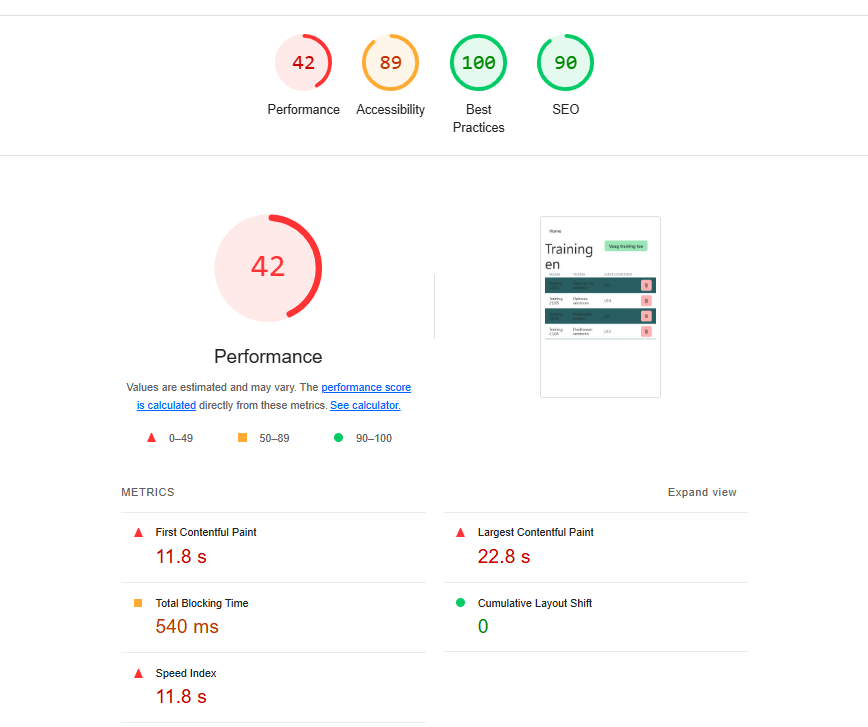
\includegraphics[width=0.3\textwidth]{JS-test1.png}
    \hfill
    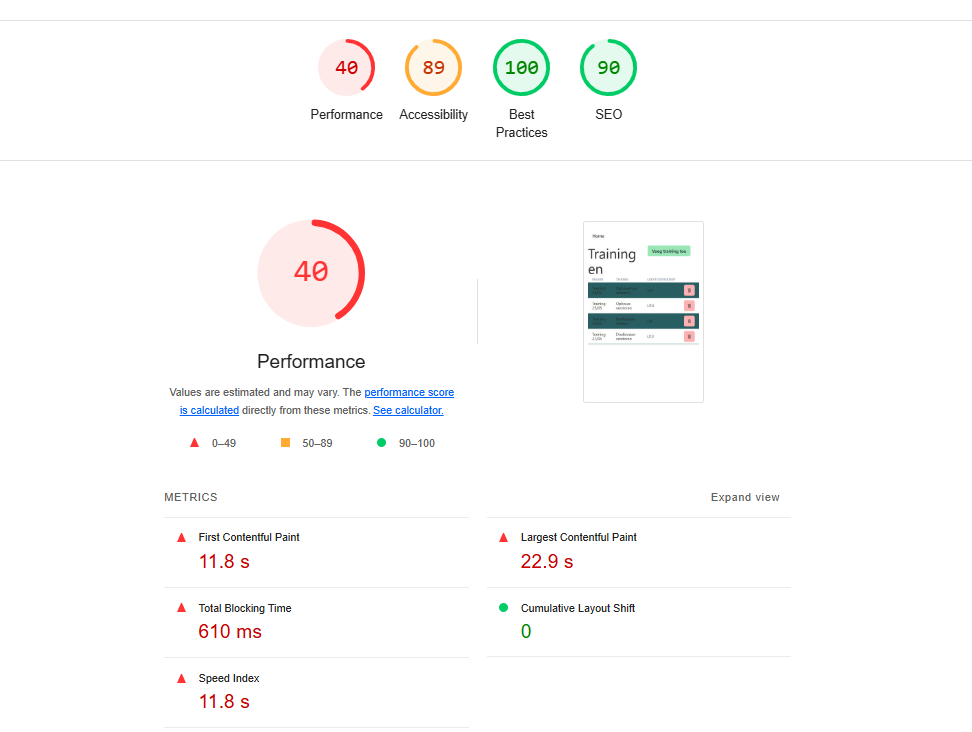
\includegraphics[width=0.3\textwidth]{JS-test2.png}
    \hfill
    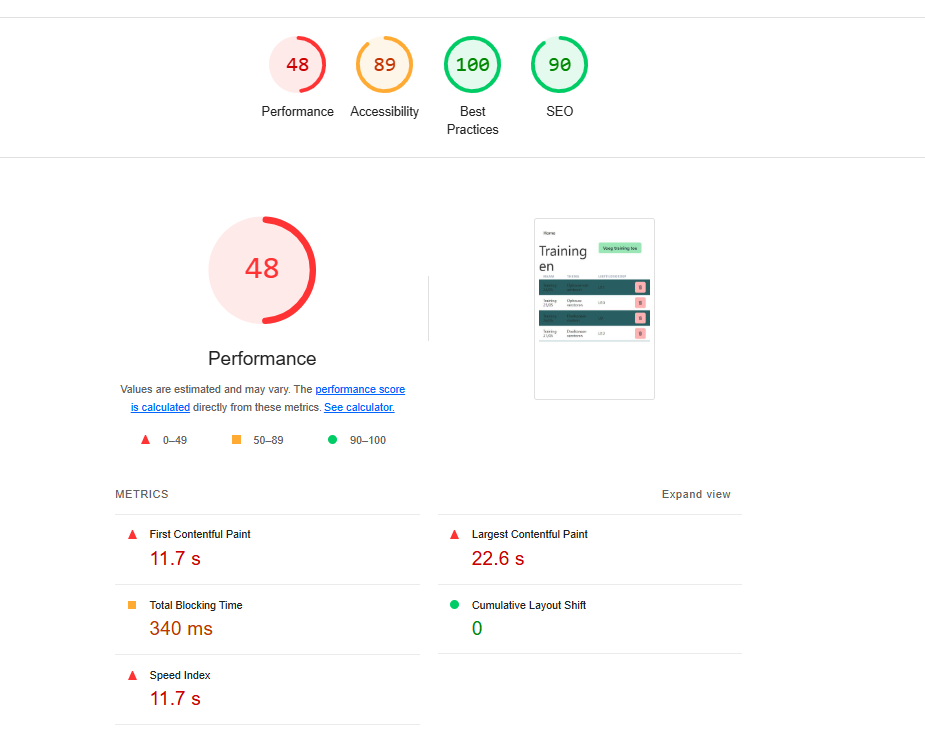
\includegraphics[width=0.3\textwidth]{JS-test3.png}
    \caption{Lighthouse testresultaten JavaScript/React - Links: Test 1, Midden: Test 2, Rechts: Test 3}
    \label{fig:javascript-simple}
\end{figure}

\newpage
\paragraph{Mendix}

\begin{table}[h]
    \centering
    \begin{tabular}{ |p{3cm}|p{2.75cm}|p{2.75cm}|p{2.75cm}|p{2.75cm}|}
        \hline
        \textbf{Metriek} & \textbf{Test 1} & \textbf{Test 2}  & \textbf{Test 3} & \textbf{Gemiddelde}\\
        \hline
        \textbf{\gls{FCP}}  & 13.7s & 13.9s & 13.7s & 13.8s \\
        \hline
        \textbf{\gls{LCP}} & 17.8s & 18.2s & 17.8s & 17.9s\\
        \hline
        \textbf{\gls{TBT}}  & 330ms & 500ms & 260ms & 363ms \\
        \hline
        \textbf{Speed Index}  & 13.7s & 13.9s & 13.7s & 13.8s \\
        \hline
        \textbf{\gls{CLS}}  & 0 & 0  & 0 & 0 \\
        \hline
        \textbf{Performance Score}  & 48 & 43  & 50 & 47 \\
        \hline
    \end{tabular}
    \caption[\centering Testresultaten laadtijd Mendix]{\label{tab:Testresultaten Mendix}Testresultaten Mendix}
\end{table}

\begin{figure}[htbp]
    \centering
    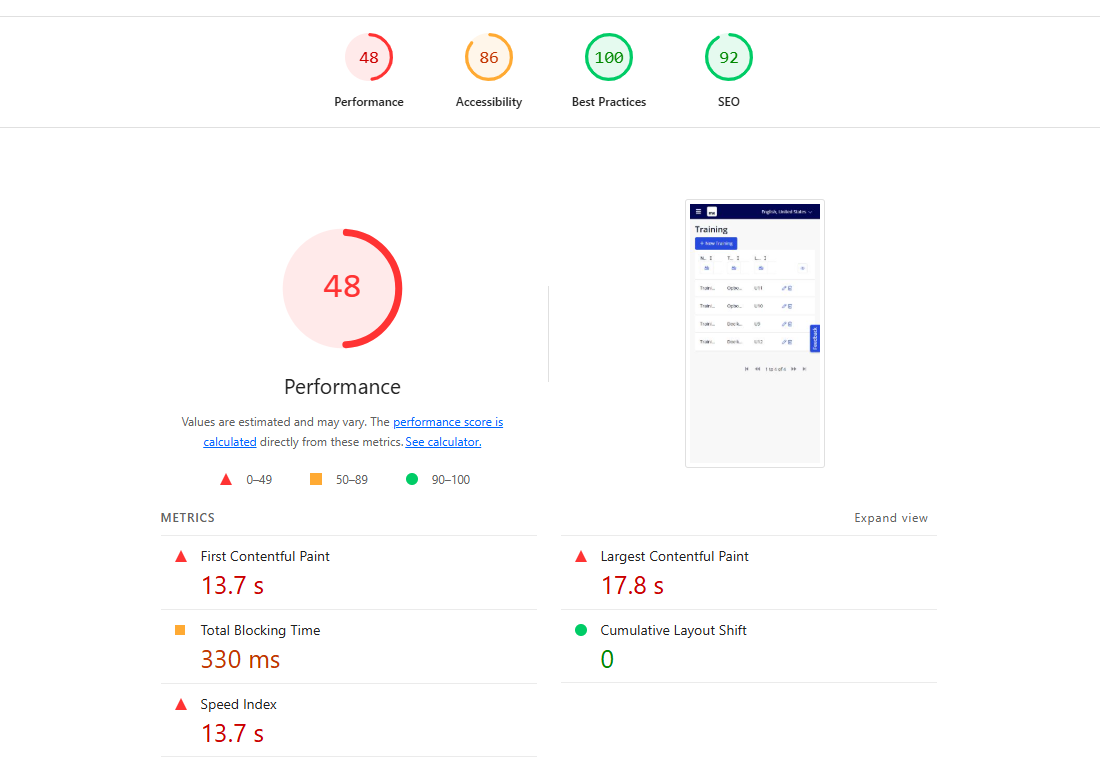
\includegraphics[width=0.3\textwidth]{Mendix-test1.png}
    \hfill
    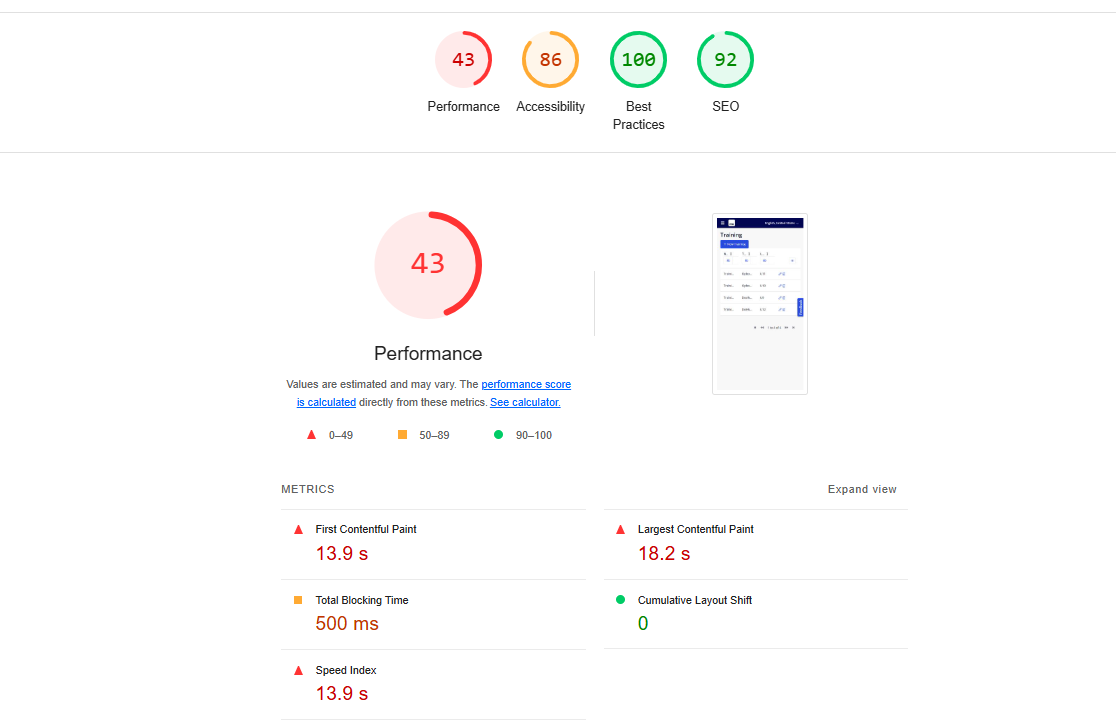
\includegraphics[width=0.3\textwidth]{Mendix-test2.png}
    \hfill
    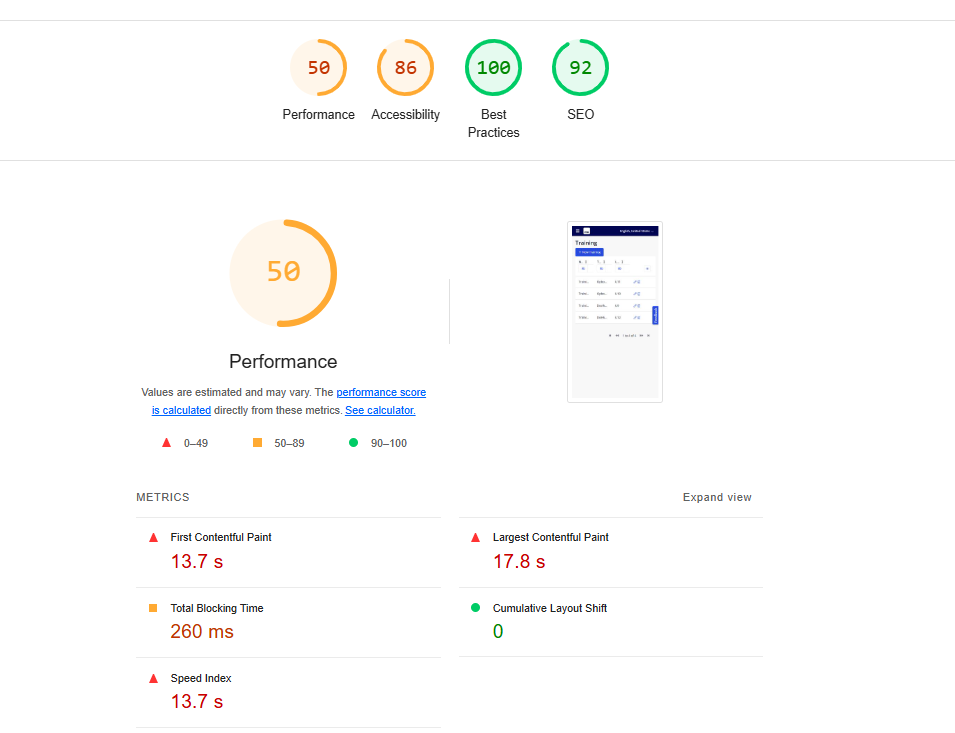
\includegraphics[width=0.3\textwidth]{Mendix-test3.png}
    \caption{Lighthouse testresultaten Mendix - Links: Test 1, Midden: Test 2, Rechts: Test 3}
    \label{fig:mendix-simple}
\end{figure}
\newpage
\paragraph{Vergelijkingstabel}
\begin{table}[h]
    \centering
    \begin{tabular}{ |p{3cm}|p{2.25cm}|p{2.25cm}|p{2.25cm}|p{3.25cm}|}
        \hline
        \textbf{Metriek} & \textbf{JavaScript/} \newline \textbf{React} & \textbf{Mendix}  & \textbf{Verschil} & \textbf{Beste Prestatie}\\
        \hline
        \textbf{\gls{FCP}}  & 11.8s & 13.8s & -2.0s & JavaScript/React \\
        \hline
        \textbf{\gls{LCP}} & 22.8s & 17.8s & +4.9s & Mendix\\
        \hline
        \textbf{\gls{TBT}}  & 497msms & 363ms & +134ms & Mendix \\
        \hline
        \textbf{Speed Index}  & 11.8s & 13.8s & -2.0s & JavaScript/React \\
        \hline
        \textbf{\gls{CLS}}  & 0 & 0  & Gelijk & Gelijk \\
        \hline
        \textbf{Performance Score}  & 43 & 47  & -4 & Mendix \\
        \hline
    \end{tabular}
    \caption[\centering Vergelijkingstabel laadtijd]{\label{tab:Vergelijkingstabel laadtijd}Vergelijkingstabel laadtijd}
\end{table}

\paragraph{Samenvatting}
\begin{itemize}
    \item JavaScript/React is sneller bij \gls{FCP} en Speed Index (2s sneller)
    \item Mendix presteert beter bij \gls{LCP} (4,9s sneller) en \gls{TBT} (134ms minder)
    \item Mendix heeft een hogere Performance Score (47 vs 43)
    \item Beide platforms hebben perfecte \gls{CLS} scores
    \item Beide platforms scoren onder acceptabele performance niveaus (<50)
\end{itemize}
De prestatieverschillen tussen Mendix en JavaScript/React kunnen verklaard worden door fundamentele verschillen in architectuur en uitvoering. JavaScript/React scoort beter op \gls{FCP} doordat het doorgaans gebruikmaakt van een lichte initiële bundel en client-side rendering, waardoor visuele elementen snel zichtbaar zijn. Mendix presteert daarentegen beter op \gls{LCP} en \gls{TBT} dankzij de geïntegreerde backend, geoptimaliseerde dataverwerking en beperkte client-side JavaScript. Door logica server-side af te handelen en automatisch platformoptimalisaties toe te passen, vermindert Mendix de belasting op de browser, wat resulteert in betere prestaties bij het laden van grote elementen en minder blokkeringen tijdens interacties.

\subsubsection{Reactietijd op gebruikersacties}
TODO
\\
Test: Meet de tijd tussen een gebruikersactie (zoals klikken op een knop) en het voltooien van de respons (bijvoorbeeld ophalen van data).

Tool: Browser performance tools
\subsubsection{Load test/ Stress test}
TODO
\\
Test: Voer een load test uit om te zien hoe de applicaties presteren bij een groot aantal gelijktijdige gebruikers.

Tool: Apache JMeter

Doel: Maximaal aantal gelijktijdige gebruikers dat de applicatie aankan voordat performance degradeert.

\subsection{Ontwikkelsnelheid en onderhoud}

\subsubsection{Ontwikkeltijd}
TODO
\\
Test: Vergelijk de daadwerkelijke tijd (in uren/dagen) die nodig was om beide applicaties te bouwen.

Meting: Handmatig loggen van ontwikkelingstijd.

Doel: Beoordelen welke stack sneller resultaat oplevert.
\subsubsection{Herbruikbaarheid / uitbreidbaarheid}
TODO
\\
Test: Voeg een nieuwe feature toe (zoals een zoekfunctie, filter, of grafiek) en meet hoeveel tijd en code nodig is.

Doel: Evaluatie van aanpasbaarheid en herbruikbaarheid van componenten.


\subsection{Integratiemogelijkheden}
Mendix is ontworpen om gemakkelijk te kunnen integreren met zowel moderne als legacy systemen. De belangrijkste integratietechnieken en mogelijkheden zijn:
\begin{itemize}
    \item \textbf{REST API's}
    \\
    Mendix biedt volledige ondersteuning voor het bouwen en gebruiken van RESTful API's. Je kunt makkelijk data van externe systemen ophalen of je eigen services beschikbaar maken voor anderen.
    Bijvoorbeeld: integreren met een CRM zoals Salesforce of een ERP zoals SAP.
    \item \textbf{SOAP Webservices}
    \\
    Ook oudere webservices (SOAP) worden ondersteund, wat belangrijk is voor legacy systemen.
    Bijvoorbeeld: communicatie met oudere financiële software of verzekeringssystemen.
    \item \textbf{GraphQL ondersteuning}
    \\
    Hoewel GraphQL niet natively wordt aangeboden zoals REST/SOAP, kan Mendix met plugins en uitbreidingen GraphQL endpoints benaderen.
    \item \textbf{OData Services}
    \\
    Voor standaardisatie en eenvoudige integratie met analytische tools (bijvoorbeeld Power BI) ondersteunt Mendix OData publicatie en consumptie.
\end{itemize}
Mendix biedt uitgebreide integratiemogelijkheden met externe systemen, API’s en databases. Het platform ondersteunt integratie via REST, SOAP, OData, GraphQL en JDBC. Daarnaast kunnen ontwikkelaars gebruikmaken van Mendix Connect en de Mendix Marketplace om connectors te vinden of te bouwen voor systemen zoals SAP, Salesforce en Kafka. Voor database-integratie biedt Mendix ondersteuning voor directe JDBC-verbindingen met databases zoals Microsoft SQL, MySQL, Oracle, PostgreSQL en Snowflake.

\subsection{Aanpasbaarheid en uitbreidbaarheid}
Het Mendix-platform is zeer aanpasbaar en uitbreidbaar. Ontwikkelaars kunnen aangepaste functionaliteiten implementeren via Java-acties, pluggable widgets (op basis van React of JavaScript) en de Mendix Model SDK. Daarnaast kunnen ontwikkelaars het platform uitbreiden met behulp van de Extensibility API, waarmee nieuwe functionaliteiten aan Studio Pro kunnen worden toegevoegd.

\subsection{Ontwikkelingssnelheid}
Mendix staat bekend om zijn snelle ontwikkelingsmogelijkheden. Het platform maakt gebruik van een visuele ontwikkelomgeving, herbruikbare componenten en een geïntegreerde CI/CD-pijplijn, wat bijdraagt aan een verhoogde ontwikkelsnelheid. Volgens \textcite{MxTechies} kunnen applicaties tot 10 keer sneller worden gebouwd met 70\% minder middelen. 

\subsection{Beveiliging en compliance}
Mendix hecht veel waarde aan beveiliging en compliance. Het platform biedt uitgebreide beveiligingsmaatregelen, waaronder toegangsbeheer, gegevensversleuteling en ondersteuning voor beveiligingsstandaarden. Daarnaast ondersteunt Mendix de opslag van applicatiegegevens in SQL-databases naar keuze, wat organisaties flexibiliteit biedt in gegevensbeheer en compliance. 
\\
\\
\subsection{Conclusie}
De uitgevoerde tests tonen aan dat Mendix een krachtig en flexibel low-code platform is dat geschikt is voor het bouwen van schaalbare, geïntegreerde en veilige applicaties. De uitgebreide integratiemogelijkheden, aanpasbaarheid en snelle ontwikkelcyclus maken het platform bijzonder geschikt voor diverse bedrijfsbehoeften.


\section{Reflectie op eigen ervaringen}
Op basis van mijn ervaring kan ik bevestigen dat low-code, zoals Mendix, bijzonder krachtig is voor het snel opzetten van generieke applicaties met standaardfunctionaliteiten. Het stelt je in staat om in korte tijd werkende oplossingen te bouwen, wat vooral in iteratieve of proof-of-concept contexten een grote meerwaarde biedt. Tegelijk merk ik dat zodra een project meer ‘custom’ noden heeft – zoals complexe bedrijfslogica of verfijnde integraties – de grenzen van het platform sneller voelbaar worden. In die gevallen is het een duidelijke troef om een high-code achtergrond te hebben: je begrijpt beter wat er onder de motorkap gebeurt, kunt gerichter zoeken naar workarounds en neemt bewuster beslissingen over de architectuur van je oplossing. Bovendien zie ik dat een traditionele programmeerachtergrond ook de leesbaarheid en structuur van je low-code logica ten goede komt. Je denkt in patronen, zorgt voor herbruikbaarheid en hanteert best practices die niet vanzelfsprekend zijn in een puur visuele ontwikkelomgeving.

\subsection{Reflectie op ervaringen van experts}
Er zijn ook enkele ontwikkelaars met een klassieke high-code achtergrond die inmiddels volledig actief zijn binnen low-code projecten, met name op het Mendix-platform. Ik sprak met hen over hun ervaringen en vatte hun bevindingen samen. 
Ze benadrukken dat low-code bijzonder krachtig is voor het snel ontwikkelen van generieke applicaties met standaardfunctionaliteiten. Dit maakt het ideaal voor situaties waarin snelheid en iteratieve ontwikkeling belangrijk zijn. Daarnaast wordt low-code vaak gepositioneerd als een brug tussen IT en business, doordat ook gebruikers zonder programmeerervaring relatief snel aan de slag kunnen. In de praktijk leidde dit er echter soms toe dat businessgebruikers eigen applicaties opstartten die later door ervaren ontwikkelaars moesten worden overgenomen. Deze overdracht bleek niet altijd evident: de onderliggende logica bleek vaak moeilijk leesbaar en voldeed zelden aan gangbare ontwikkelstandaarden of best practices, wat extra werk met zich meebracht om de applicatie te stabiliseren en verder te ontwikkelen.

Wat betreft de ontwikkelervaring binnen Mendix, werd er gemengd gereageerd op de version control-functionaliteit. Hoewel het systeem in principe krachtig is en goed integreert met teamwerk, kunnen foutmeldingen en merge-conflicten soms moeilijk te doorgronden zijn. Wanneer alles echter correct functioneert, biedt het versiebeheer een betrouwbare en efficiënte manier van samenwerken. De integratie van agile werkmethodieken binnen het Mendix-platform werd unaniem positief beoordeeld: user stories, sprints en voortgang kunnen rechtstreeks via de projectpagina opgevolgd en beheerd worden, wat de samenwerking tussen ontwikkelaars en stakeholders vergemakkelijkt.

Ook het gebruik van herbruikbare modules uit de Mendix Marketplace werd als een groot voordeel genoemd. Het toevoegen van bestaande componenten versnelt de ontwikkeling aanzienlijk en voorkomt dat het wiel telkens opnieuw moet worden uitgevonden. Tegelijk wordt opgemerkt dat een groot aantal van deze modules weinig tot geen documentatie bevat, waardoor het tijd kost om hun werking te doorgronden of aan te passen aan specifieke projectbehoeften. 

Over het geheel genomen beschouwen deze ontwikkelaars Mendix als een toegankelijke en efficiënte ontwikkelomgeving, die eenvoudig aanvoelt in de basis, maar bij complexere noden ook de nodige technische diepgang vereist. Hun ervaring met high-code vormt daarbij een duidelijke meerwaarde: het helpt hen om concepten sneller te begrijpen, kwalitatieve oplossingen te bouwen en de leesbaarheid en onderhoudbaarheid van hun low-code toepassingen te verbeteren.

\section{Evaluatie van Mendix-uitbreidingen}
Op basis van gesprekken met ervaren ontwikkelaars die dagelijks met Mendix werken, blijkt dat het gebruik van standaard Marketplace-modules doorgaans als efficiënt en tijdbesparend wordt ervaren, vooral bij generieke functionaliteiten. Deze modules kunnen snel geïntegreerd worden, wat de implementatietijd aanzienlijk verkort. Toch werd ook opgemerkt dat veel van deze modules onvoldoende of zelfs geheel geen documentatie bevatten. Dit gebrek aan transparantie leidt tot vertragingen tijdens implementatie en beperkt de flexibiliteit wanneer aanpassingen nodig zijn. In zulke gevallen biedt custom ontwikkeling vaak meer controle en beter afgestemde oplossingen, hoewel dit uiteraard gepaard gaat met een langere ontwikkeltijd en hogere initiële kosten.

Java-uitbreidingen binnen Mendix worden door ontwikkelaars met een high-code achtergrond beschouwd als waardevolle tools om de beperkingen van het platform te omzeilen, bijvoorbeeld bij complexe logica of integraties met externe systemen. Deze uitbreidingen verhogen echter ook de technische complexiteit van het project en kunnen de onderhoudbaarheid op lange termijn negatief beïnvloeden, zeker wanneer ze niet goed gedocumenteerd zijn of slechts door een beperkte groep binnen het team begrepen worden.

Wat betreft de kosten-batenverhouding, geven ontwikkelaars aan dat low-code in combinatie met herbruikbare modules initieel voordeliger is in zowel ontwikkeling als beheer. Naarmate de applicatie complexer wordt en meer ‘maatwerk’ vereist, verschuift dit evenwicht echter, en kunnen custom uitbreidingen of Java-integraties duurder uitvallen, zowel in termen van ontwikkeluren als bij latere aanpassingen of onderhoud.

Tot slot werd ook het integreren van externe systemen als een uitdaging benoemd. Hoewel Mendix hier voldoende ondersteuning voor biedt, vergt het combineren van low-code met externe services een goed begrip van beide kanten. Een technische achtergrond blijkt in die context bijzonder waardevol, zowel voor het begrijpen van de externe API’s als voor het bouwen van robuuste, onderhoudbare koppelingen binnen het platform. Al met al tonen deze bevindingen aan dat een doordachte strategie, met oog voor schaalbaarheid en onderhoud, essentieel is bij het uitbreiden van Mendix-toepassingen.

\section{Ontwikkeling beslissingskader}
TODO
\\
\\
Voor het beantwoorden van deelvraag 8, die zich richt op het destilleren van best practices en richtlijnen voor de keuze tussen Mendix en traditionele ontwikkeling, wordt een gestructureerd beslissingskader ontwikkeld. Dit kader ondersteunt projectmanagers en architecten bij het maken van weloverwogen keuzes over de inzet van Mendix in vergelijking met conventionele ontwikkelmethoden. Het biedt beslissingspunten voor de initiële keuze tussen Mendix en traditionele ontwikkeling en stelt criteria vast om te bepalen welke projectonderdelen beter geschikt zijn voor high-code ontwikkeling. Daarnaast worden richtlijnen geformuleerd voor het effectief combineren van low-code en high-code in hybride projecten, zodat beide benaderingen optimaal kunnen worden ingezet. Verder bevat het kader aanbevelingen voor de vroege identificatie van potentiële beperkingen en risico’s, waardoor projectrisico’s proactief kunnen worden gemitigeerd. Tot slot worden strategieën ontwikkeld om op basis van eerdere ervaringen en literatuur weloverwogen keuzes te maken bij toekomstige projecten. Dit beslissingskader draagt bij aan een systematische en onderbouwde aanpak voor het selecteren van de meest geschikte ontwikkelmethode binnen uiteenlopende projectcontexten.


